\documentclass[light]{lutbeamer} % change between light and dark for the background
%\documentclass[t]{lutbeamer} % use "t" option for top alignment 
\usepackage{caption}
\usepackage{xcolor}
\captionsetup{labelfont={color=gr},textfont={color=gr}}
\DeclareCaptionLabelFormat{nocolon}{#1 #2}
\captionsetup{labelformat=nocolon}
\usepackage{pgfpages}
\usepackage{amssymb}
\usepackage{amsmath}
\usepackage{tabularx}
\usepackage{array}
\usepackage{adjustbox}
\usepackage{hyperref} % Link
\usepackage{bm}
\usepackage{amsfonts}
\usepackage{algorithmic}
\usepackage{textcomp}
\usepackage{xcolor}
\usepackage{algorithm} 
\usepackage{amsthm} % add this package to use the definition environment

\setbeameroption{hide notes} % Only slides
% \setbeameroption{show only notes} % Only notes
% \setbeameroption{show notes on second screen=right} % Both


% Define the custom color using hexadecimal code
\definecolor{customcolor}{HTML}{123363}

% Define a new block environment with a custom background color and white text
\newenvironment{customblock}{%
    \setbeamercolor{block body}{bg=customcolor,fg=white}%
    \begin{block}%
}{%
    \end{block}%
}


\setdepartment{Data Science and Analytics Thrust, Information Hub}
\institute[HKUSTGZ]{The Hong Kong University of Science and Technology (Guangzhou)}
\author{Mingze Gong}
\title{Spatio-Temporal Forecasting}
\subtitle{Deterministic Graph Neural Networks for Carbon Emissions and Generative Probabilistic Stochastic Differential Equation-based Diffusion for Traffic Flow}
\date{\today}


\begin{document}

% % front page
% { % all template changes are local to this group.
% \setbeamertemplate{navigation symbols}{}
% \begin{frame}<article:0>[plain,noframenumbering]
%     \begin{tikzpicture}[remember picture,overlay]
%         \node[at=(current page.center)] {
%             \includegraphics[
%                 width=\paperwidth,
%                 height=\paperheight]{figures/GZ Campus.jpeg}
%         };
%     \end{tikzpicture}
% \end{frame}
% }

% Outline with figure on the right
\AtBeginSubsection[]
{
    \begin{frame}[plain,noframenumbering]
        \frametitle{Outline}
        \begin{columns}
            % Left column for the outline
            \begin{column}{0.6\textwidth}
                \tableofcontents[currentsection,
                    currentsubsection,
                    %hideothersubsections, 
                    %sectionstyle=show/shaded, 
                    %subsectionstyle=show/shaded%/hide
                ]
            \end{column}
            \hspace{-4em}
            % Right column for the figure
            \begin{column}{0.42\textwidth}
                \begin{figure}
                    \centering
                    \vspace{-2em}
                    \includegraphics[width=\textwidth]{logos/GZ Campus.pdf} % Adjust path and filename
                \end{figure}
            \end{column}
        \end{columns}
    \end{frame}
}


{ % title page
    \begin{frame}[plain]
        \maketitle
        \small
        \par\vskip-0.1em
        {\footnotesize
        \begin{beamercolorbox}[sep=8pt,left]{author}
            \usebeamerfont{author}{Presented by \insertauthor} on \insertdate
        \end{beamercolorbox}%\vskip0.5em
        }
    \end{frame}
}
% % % % % % % % % % % % % % % % % % % % % % % % % % % % % % % % % % % %
\section{Research Questions in the Paper}
% \subsection{Research Overview}
\begin{frame}
    \frametitle{Research Questions in the Paper}
    \framesubtitle{Feeder}

    What real-time data/information can be gained  from the LiW feeder signals that relate to changes in  powder properties beyond mass flow?

    \begin{itemize}
        \item \textbf{Context:} LiW feeders control mass flow rates of powders, essential for continuous manufacturing precision.
        \item \textbf{Signals Indicators:} Changes in screw speed, motor torque, and weight fluctuations may reflect variations in:
              \begin{itemize}
                  \item Density
                  \item Particle size
                  \item Flowability
              \end{itemize}
        \item \textbf{Goal:} Utilize feeder signal variations to infer real-time changes in powder properties, improving product quality and process consistency.
    \end{itemize}
\end{frame}



% % % % % % % % % % % % % % % % % % % % % % % % % % % % % % % % % % % %
% % % % % % % % % % % % % % % % % % % % % % % % % % % % % % % % % % % %
% % % % % % % % % % % % % % % % % % % % % % % % % % % % % % % % % % % %
% % % % % % % % % % % % % % % % % % % % % % % % % % % % % % % % % % % %
% % % % % % % % % % % % % % % % % % % % % % % % % % % % % % % % % % % %
% % % % % % % % % % % % % % % % % % % % % % % % % % % % % % % % % % % %
% % % % % % % % % % % % % % % % % % % % % % % % % % % % % % % % % % % %
% % % % % % % % % % % % % % % % % % % % % % % % % % % % % % % % % % % %

\appendix % to start a separate page numbering

\section*{Bibliography}
\begin{frame}[allowframebreaks]
    \textbf{References}
    \printbibliography
\end{frame}


{ % all template changes are local to this group.
\setbeamertemplate{navigation symbols}{}
\begin{frame}<article:0>[plain,noframenumbering]
    \begin{tikzpicture}[remember picture,overlay]
        \node[at=(current page.center)] {
            
\includegraphics[
                width=\paperwidth,
                height=\paperheight]{logos/ThankYouPage.png}
        };
    \end{tikzpicture}
\end{frame}
}

\end{document}
